%*****************************************
\chapter{Lab 05: Explore}\label{ch:lab05}
%*****************************************
%\setcounter{figure}{10}
%\NoCaseChange{Homo Sapiens}
%\listoftodos % Creates the ToDo listing

\section{Introduction}

Preparing and ``cleaning'' data before it is used in statistical analysis is an important and time-consuming process. It should make sense that to find a mean of a data element is rather pointless if that element contains bad data. While the process of cleaning data is beyond the scope of this manual there are a few simple steps researchers can take to attempt to verify the integrity of the data. This lab examines the \acs{PSPP} \textit{Explore} feature that permits that sort of examination.

\section{Discussion}

\subsection{Data Problems}

There are a number of simple tests that researchers can perform on a data element before they start working with it to determine if there are problems that may foul further statistical analysis. While some data analysis programs include tools to help clean and prepare data for analysis it is probably better to use software that has been specifically created for that purpose so the data can be ready before it is ever imported into a program like \acs{PSPP}. For students who want to explore this aspect of data analysis, \href{http://openrefine.org/}{Open Refine} is an excellent place to start. This was formerly \textit{Google Refine} and is an easy-to-use, but powerful, data preparation tool with a many free online tutorials and other help.

\subsubsection{Data Element Type}

When data are first imported into the data base it is possible for the automatic process to misidentify the type of data being imported. For example, a numeric data element may be imported as text and that would limit the types of analysis that could be completed. This type of error is normally very easy to detect and correct by simply changing the data element's attribute settings.

\subsubsection{Duplicate Data}

Often records in a dataset are duplicated and this would create a problem when analyzing the data. Some data analysis software includes built-in procedures to detect and correct duplicate data, but this type of error can more efficiently be corrected with data preparation software made to correct these errors.

\subsubsection{Missing Data}

Often, survey data will have missing values because the respondents did not complete one or more questions for some reason. This creates missing data and researchers need to account for those missing items. There are several techniques used to allow for missing data.

\begin{itemize}
  \item Ignore records. It is possible to simply exclude an entire record from analysis if there are any missing elements within that record. This should only be done if the number of records being excluded is less then 5\% of the total number of records. Excluding records also does not work well for data from matched trials (``before/after'' types of experiments) or time values (where something is being measured over a long period of time).
  \item Setting missing values to a fixed value. It is possible to simply find-replace all missing values with some fixed number, like $ 0 $. This, though, leads to a number of additional problems and should not be used.
  \item Estimating values. It is common to replace missing values with an estimate for the missing data. For example, missing values could be replaced by the mean of the entire dataset or by the mean that is calculated from nearby values.
\end{itemize}

\subsubsection{Outliers}

It is common for interval and ratio data to include outliers, or values that are far outside the range of ``normal'' values. For example, a survey of home prices in a neighborhood may reveal that the mean value of a home is \$150K but there is one mobile home in the neighborhood that is valued at only \$75K. That low value would be an outlier that would concern researchers.

There are several methods used to deal with outliers. If there is an obvious coding error, like a decimal point in the wrong place, then it can simply be corrected. Outliers can also be systematically changed to a value that is three standard deviations from the mean. They can also be excluded from analysis by using a method like trimmed means. Finally, if the outliers seem to contain data that is important for further analysis, then the dataset can be split such that the outliers end up in their own subset where they can receive more scrutiny.

\subsubsection{Data Distribution}

Most statistical tests require data to be normally distributed and if the dataset has some other distribution, or is badly skewed or shows an abnormal kurtosis\footnote{Lab 1 contains information on data distributions, skew, and kurtosis.}, then the statistical analysis may fail. To try to correct the distribution it is possible to apply some sort of transformation to the data to see if a better fit can be achieved. As one example, the common logarithm can be taken of the data and that may fit a normal distribution curve better than the raw data.

\section{Procedure}

%TODO Nice definition: Confidence intervals are ranges where the true mean is expected to lie. 

\subsection{Data Element Type}

The simplest way to check and correct an improperly imported data error is to examine the attributes for the data elemets to see if they seem to be correct. Within \acs{PSPP}, click \textsc{\fbox{Variable View}} at the bottom of the data window and look carefully at each variable's attributes.

\begin{figure}[H]
  \begin{center}
    \fbox{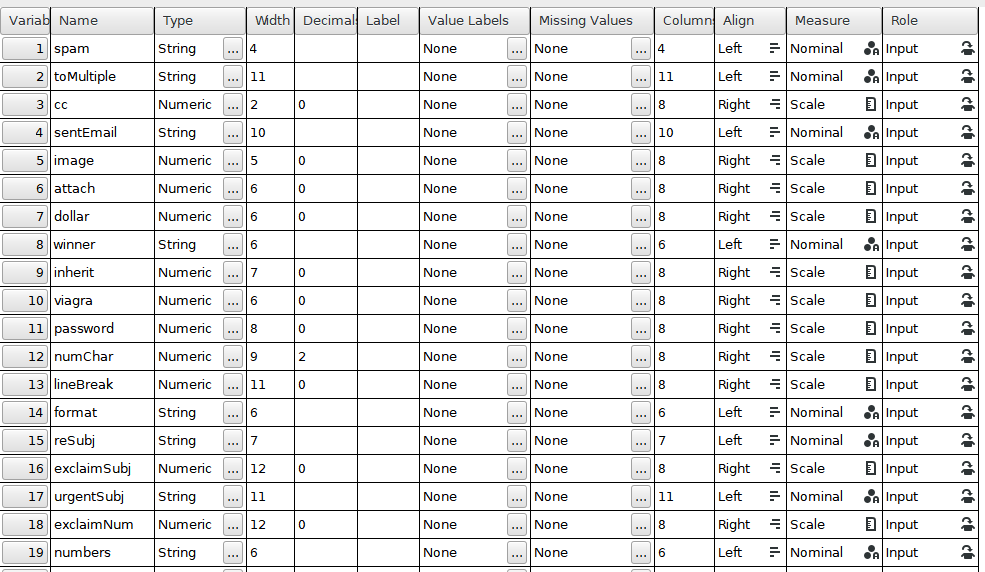
\includegraphics[width=\linewidth]{gfx/Lab05_fig01}}
    \caption{Attributes for the Email Dataset Elements}
    \label{lab05_fig01}
  \end{center}
\end{figure}

In Figure \ref{lab05_fig01}, the type of data is found in column three and that can be changed if necessary. The data width is found in columns four and five where string data (that is, text data) is restricted to only the number of characters in column four. For numeric data the integer part is restricted to the width specified in column four and the decimal to that specified in column five. The other column of interest is $ 11 $, labeled ``Measure.'' That indicates how the data are being used by \acs{PSPP} and that can be easily changed between Nominal, Ordinal, and Scale (that is both ratio and interval).

\subsection{Duplicate Data}

\acs{PSPP} does not include a method to detect duplicate data; therefore, a pre-processing program, like \href{http://openrefine.org/}{Open Refine} should be used to prepare the dataset, include removing duplicate records, before it is imported.

\subsection{Missing Data}

Start \acs{PSPP} and open the \textit{births} dataset, then:

\begin{enumerate}
  \item Click \textsc{\fbox{Analyze $ \rightarrow $ Descriptive Statistics $ \rightarrow $ Explore}}
  \item Click the word \textit{visits} in the left column and then click the right-arrow button near the center of the window to move \textit{visits} to the ``Dependent List'' box on the right side of the window. (Alternatively, double-click the word \textit{visits} in the left column to move it to the ``Dependent List'' box.)
  \item Click \textsc{\fbox{Statistics}} at the bottom of the screen.
  \item Select all three statistics functions: Descriptives, Extremes, and Percentiles.
  \item Click \fbox{Continue} to close the Statistics window.
  \item Click \fbox{OK} to generate the requested information.
\end{enumerate}

\begin{figure}[H]
  \begin{center}
    \fbox{\includegraphics[width=\linewidth]{gfx/lab05_fig03}}
    \caption{Generating Explore Information}
    \label{lab05_fig03}
  \end{center}
\end{figure}

\begin{figure}[H]
  \begin{center}
    \fbox{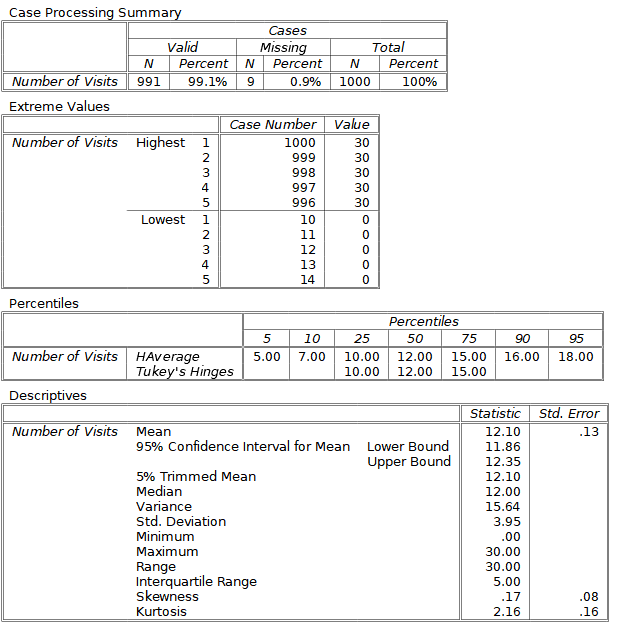
\includegraphics[width=\linewidth]{gfx/lab05_fig04}}
    \caption{Explore Information}
    \label{lab05_fig04}
  \end{center}
\end{figure}

The ``Case Processing Summary'' box at the top of Figure \ref{lab05_fig04} indicates that the \textit{age} element is missing nine cases, which is only about $ 0.9\% $ of the total number of cases in the dataset. Becuase this is well under $ 5\% $ of the total number of cases, it would be reasonable to simply ignore the missing cases if the \textit{visits} data were being analyzed.

\subsection{Activity 1: Missing Data} \label{lab05_act01}

Using the \textit{births} dataset, determine the number and percent of missing cases for \textit{Father's Age} and \textit{Weight Gained}.

\subsection{Outliers}

There is no rigid statistical definition of ``outlier'' so there is no one way to detect them. However, there are several simple techniques can be used to determine if a data element has suspected outliers. 

``Tukey's Test'' is to take the Interquartile Range (IQR) and multiply that by $ 1.5 $ then subtract that number from the first quartile and add it to the third quartile. Any values that lie outside those boundaries should be investigated as potential outliers. As an example, consider Figure \ref{lab05_fig04}.

\begin{enumerate}
  \item The IQR of $ 5.00 $ is found in the ``Descriptives'' table.
  \item Multiply the IQR by $ 1.5 $ to get $ 7.5 $.
  \item The values of the first ($ 25\% $) and third ($ 75\% $) quadrants are found in the ``Percentiles'' box.
  \item Subtract $ 10.00 - 7.5 $ to get the lower bound of $ 2.5 $.
  \item Add $ 15.00 + 7.5 $ to get the upper bound of $ 22.5 $.
  \item Use the ``Extreme Values'' box to see if any values lie below the lower bound or above the upper bound and there are many.
\end{enumerate}

Another approach is to look for values that are more than three standard deviations from the mean of the dataset. Again, using Figure \ref{lab05_fig04}:

\begin{enumerate}
  \item The mean of $ 12.10 $ is found in the ``Descriptives'' table.
  \item The standard deviation of $ 3.95 $ is found in the ``Descriptives'' table.
  \item Multiply the standard deviation by $ 3 $ to get $ 11.85 $.
  \item Subtract $ 12.10-11.85 $ to get the lower bound of $ 0.25 $.
  \item Add $ 12.10+11.85 $ to get the upper bound of $ 23.95 $.
  \item Use the ``Extreme Values'' box to see if any values lie below the lower bound or above the upper bound and there are many.
\end{enumerate}

It is perhaps easiest to use the Z-Score to look for outliers. Since the Z-Score is the number of standard deviations a data point lies from the mean, researchers can look for any Z-Scores above $ +3.0 $ or below $ -3.0 $ to detect outliers. The method for calculating Z-Scores with \acs{PSPP} was described on page \pageref{z-scores}. The Z-Scores for \textit{Visits} in the \textit{Births} dataset was calculated and Figure \ref{lab05_fig05} shows the top $ 19 $ and bottom $ 11 $ cases for that data element.

\begin{figure}[H]%
  \centering
  \parbox{.45\linewidth}{
    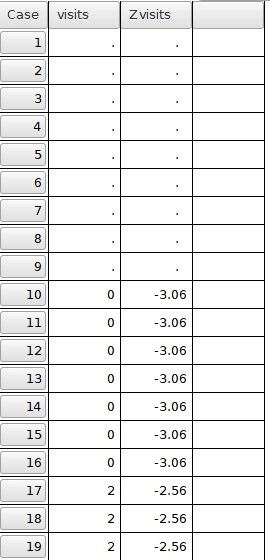
\includegraphics[width=\linewidth]{gfx/lab05_fig05}
  }%
  \qquad
  \begin{minipage}{.45\linewidth}%
    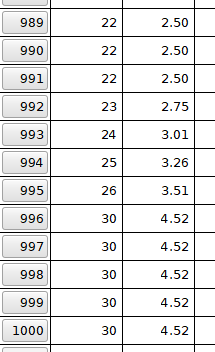
\includegraphics[width=\linewidth]{gfx/lab05_fig06}
  \end{minipage}%
  \caption{Z-Scores for Visits}%
  \label{lab05_fig05}%
\end{figure}

Notice that the top nine cases have missing data, indicated by a dot, but cases $ 10-16 $ have a Z-Score of $ -3.06 $, which are more than three standard deviations below the mean and would be likely outliers. In the same way, cases $ 993-1000 $ are all more than three standard deviations above the mean and would be likely outliers.

\subsection{Activity 2: Outliers} \label{lab05_act02}

Using the \textit{births} dataset, determine the outliers for the \textit{weight} data element. For this activity, assume that any weight that is more than three standard deviations below or above the mean is an outlier. Report the weight, the Z-Score, and number of times that weight appears in the dataset. The response should be similar to this:

\begin{table}[H]
  \begin{center}
    \begin{tabular}{ccc} 
      Weight & Z-Score & Number \\
      1.20 & -3.55 & 3 \\
      1.18 & -3.54 & 1 \\
      11.75 & +3.10 & 2 
    \end{tabular}
  \end{center}
\end{table}

\subsection{Activity 3: Outliers} \label{lab05_act03}

Using the \textit{cafe} dataset, determine the outliers for the \textit{miles} data element. For this activity, assume that any values more than three standard deviations below or above the mean is an outlier. Report the miles, the Z-Score, and number of times that value appears in the dataset. The response should be similar to the table in Activity 2.

\section{Deliverable}

Complete the following activities in this lab:

\rowcolors{1}{gray!25}{}
\begin{center}
  \begin{tabular}{lll}
    \hline 
    \textbf{Number} & \textbf{Name} & \textbf{Page} \\ 
    \hline 
    \ref{lab05_act01} & \nameref{lab05_act01} & \pageref{lab05_act01} \\ 
    \ref{lab05_act02} & \nameref{lab05_act02} & \pageref{lab05_act02} \\ 
    \ref{lab05_act03} & \nameref{lab05_act03} & \pageref{lab05_act03} \\ 
    \hline 
  \end{tabular} 
\end{center}

Consolidate the responses for all activities into a single document and submit that document for grading.
